% concatenated from maine.tex
\documentclass[11pt]{article}
\usepackage{times}
\usepackage{amsmath,amssymb}
\usepackage{theoremref}
\usepackage[utf8]{inputenc}
\usepackage{indentfirst}
\setlength{\parindent}{1em}
\usepackage{graphicx,tikz}
\pagenumbering{gobble}
\usepackage{xcolor}
\usepackage{xskak}
\usepackage[T1]{fontenc}
\usepackage{amsthm}
\newtheorem{problem}{Question}%[section]
\newtheorem{definition}[problem]{Definition}
\newtheorem{theorem}[problem]{Theorem}
\newtheorem{observation}[problem]{Observation}
\newtheorem{lemma}[problem]{Lemma}
\newtheorem{conjecture}[problem]{Conjecture}
\newtheorem{corollary}[problem]{Corollary}

\title{Torus Queen Independence}
\author{Kada Kálmán Williams}

\begin{document}

\maketitle

\begin{abstract}
    Define a queen on $\mathbb{Z}_n^d$ with admissible moves parallel to $\mathbf{x}\in\{-1,0,1\}^d$, of arbitrary length. How many queens can be placed on $\mathbb{Z}_n^d$ without any two in conflict? In two dimensions, this problem was initiated by Pólya in 1918 and resolved by Monsky in 1989. We give the first known impossibility result in $d>2$ dimensions, showing that a trivial upper bound $n^{d-1}$ cannot be achieved if $n$ is a multiple of $5$ and not of $25$. Moreover, we conjecture that $n^{d-1}-O(n^{d-2})$ queens can be placed independently, which we prove if $n$ has no prime divisor less than $2^{\lfloor d/2\rfloor +1}$.
\end{abstract}

\textbf{AMS subject classification:} 05C35, 05C69

\section{Introduction}

The sport of chess is played on an $8\times 8$ board, where various figurines occupy unique fields and move between them. A king, to begin with, moves from its field onto any of the eight fields that share a corner or an edge with it. A bishop and a rook move diagonally and horizontally or vertically, respectively. A queen can move a bishop move or a rook move -- parallel to a king move, but unbounded.

A number of journals are devoted to investigating the game theoretic aspects of chess, but we are going to relate chess to graph theory \cite{HeH}. Consider a figurine graph whose nodes are the fields of a chess board, joined by an edge if a certain figurine, such as a queen, can move between those fields.\footnote{We remark that in chess, this relation is not symmetric for pawn moves, but aside from that awkward case, a simple graph is obtained.} For such a graph as the queen graph, the inspection of certain graph parameters, e.g. the domination and independence numbers, could interest chess players and combinatorialists alike.

While there are $2n-1$ diagonals in either direction on the $n\times n$ board, if moving across the boundary is permitted, as though the board were $\mathbb{Z}\times \mathbb{Z}$ modulo $n$, there are only $n$ diagonals. We identify the fields of this modular, toroidal board with $\mathbb{Z}_n^2$ \cite{BeS}. It is well-known that $n$ queens can be placed without conflict on the $n\times n$ board \cite{Pau}, or in other words, that there is an independent set of size $n$ in the $n\times n$ queen graph. However, an independent set of $n$ queens exists on the toroidal board $\mathbb{Z}_n\times \mathbb{Z}_n$ if and only if $n\equiv \pm 1\pmod 6$ \cite{Pol}.

We may further inquire into what happens when $d=2$ is replaced with a higher dimensionality $d>2$. (For sake of completeness, we determine the independence number of the queen graph on $\mathbb{Z}_n^2$ in the Appendix, following \cite{Mon}.) In order to do that, we must specify how a queen moves on $\mathbb{Z}_n^d$. In this regard, we mention three different possible definitions. Firstly, a queen could move like a two-dimensional queen while any $n-2$ coordinates are fixed, which we refer to as a plane queen. Secondly, a queen could move along a hyperplane with normal vector in $\{-1,0,1\}^d$ \cite{Nud}, to be known as a dual queen. Thirdly, a queen could move parallel to a nonzero vector in $\{-1,0,1\}^d$ \cite{BeS}, which we simply call queen. For the first and third versions of queen, we conjecture there is a placement of $n^{d-2}(n-O(1))$ queens without conflict in $d\ge 2$ dimensions, which we prove if all prime divisors of $n$ are at most $2^{\lceil \frac{d+1}{2}\rceil}$. Furthermore, we give the first known impossibility proof concerning a queen in $d\ge 3$ dimensions, establishing that $n^2$ queens cannot be placed on $\mathbb{Z}_n^3$ without conflict if $n\equiv \pm 5,\pm 10\pmod{25}$.

\section{Constructions}

We now turn to proving lower bounds for the possible size of an independent subset of the queen graph on $\mathbb{Z}_n^d$, meaning that fields are connected with an edge in this graph if they represent a queen move. For $d=3$, Klarner \cite{Kla} showed that $n^2$ independent queens on $\mathbb{Z}_n^d$ are attainable if $n$ is coprime to all the primes up to $2^d-1=7$, and like Van Rees \cite{VaR}, we shall extend this to $d>3$ dimensions. % Building on the work of Monsky and Klarner, we obtain our main result, giving an explicit independent set of $n^{d-1}-O(n^{d-2})$ queens on $\mathbb{Z}_n^d$.



Although our definitions of a plane queen, a dual queen, and a queen coincide in $d=2$ dimensions, there is a distinction between these in $d>2$ dimensions, on $\mathbb{Z}_n^d$. Nudelman \cite{Nud} found an example of $n$ dual queens on $\mathbb{Z}_n^d$ if $n$ is coprime with $(2^d-1)!$. We give an example of $n^{d-1}$ queens on $\mathbb{Z}_n^d$ if $n$ is coprime with $(2^d-1)!$ and show that a weaker condition suffices for plane queens.

\begin{theorem}\label{dim}
On the $d$-dimensional toroidal board $\mathbb{Z}_n^d$, there is an independent set of $n^{d-1}$ queens if $n$ admits no prime factor less than $2^d$. Moreover, there is an independent set of $n^{d-1}$ plane queens if $n$ is odd and coprime with $2^j\pm 1$ for $1\le j\le d-1$.
\end{theorem}

\begin{proof}
Consider placing queens on the following lattice of $n^{d-1}$ fields:
$$\{(t_1,-2t_1+t_2,-2t_2+t_3,\ldots,-2t_{d-1}):t_1,\ldots,t_{d-1}\in \mathbb{Z}_n\}.$$
Suppose, for the sake of contradiction, that now there are two queens in conflict. By definition, this occurs if and only if their displacement vector is $\mathbf{e}\in \{-1,0,1\}^d$ scaled by $\lambda\in \mathbb{Z}_n$; in the case of plane queens, $\mathbf{e}$ has at most two nonzero coordinates. Since the lattice is defined by linear expressions, the displacement between any two fields also has this form. Hence, if two queens on these fields are in conflict, there is a nontrivial solution of
$$(t_1,-2t_1+t_2,-2t_2+t_3,\ldots,-2t_{d-1})=\lambda(e_1,e_2,\ldots,e_d).$$
In particular, $t_1=e_1 \lambda$, and by solving the recursion $-2t_{l-1}+t_l=\lambda e_l$ ($2\le l\le d$ and $t_d:=0$),
$$t_l=\lambda(e_l+2e_{l-1}+\ldots+2^{l-1} e_1),\qquad l=1,2,\ldots,d.$$
The final equation reads $0=\lambda(e_d+2e_{d-1}+\ldots+2^{d-1} e_1)$, which implies $\lambda=0$, provided the bracket is coprime with $n$. Let the first instance of a sign $\pm 1$ in the list $e_d,e_{d-1},\ldots,e_1$ occur at $e_{d-i}$. The bracket, then, is $2^i$ times an odd integer bounded by $2^0+2^1+\ldots+2^{d-1}=2^d-1$. Indeed, for plane queens, this odd integer is of the form $\pm 1$ or $\pm 1\pm 2^j$. Hence, if $n$ has no prime factor less than $2^d$, then the number in the bracket is coprime with $n$, and contradiction ensues. For plane queens, it suffices for $n$ to be odd and coprime with $2^j\pm 1$, where $1\le j\le d-1$.
\end{proof}

\textbf{Remark.} While it is possible to place $n$ independent queens on an $n\times n$ board for $n\ge 4$, it is unknown whether $n^2$ independent queens can be placed on an $n\times n\times n$ board for sufficiently large $n$. For small cases, Kunt \cite{Kun} gave a computational proof that if $1\le n\le 14$, this can only be done for $n=11$ or $n=13$. 

Klarner \cite{Kla} showed the $n^2$ queens on $(t_1,t_2,3t_1+5t_2)\in \mathbb{Z}_n^3$ are independent for these values of $n$, and Van Rees generalised this observation to $d$ dimensions \cite{VaR}, \cite{Kun}. However, our example in Theorem \ref{dim} adapts well to plane queens, and we will make use of it when constructing independent sets of $n^2-O(n)$ queens in $\mathbb{Z}_n^3$, where $n$ is not a multiple of $2$ or $3$.

\begin{conjecture}\label{dimqueens}
There is an independent set of $n^{d-1}-O(n^{d-2})$ queens on $\mathbb{Z}_n^d$.
\end{conjecture}

Analogously, Nudelman \cite{Nud} conjectured that for each dimensionality $d$, $n-O(1)$ many dual queens can be placed on $\mathbb{Z}_n^d$ without conflict.

By modifying the construction we gave to prove Theorem \ref{dim}, we can confirm the claim of Conjecture \ref{dimqueens} in the case that $n$ admits no prime factor less than $2^{\lfloor d/2\rfloor +1}$.

\begin{theorem}\label{dqueens}
For any $d\ge 3$, on the $d$-dimensional toroidal board $\mathbb{Z}_n^d$, there is an independent set of $n^{d-1}-O(n^{d-2})$ queens if the smallest prime factor of $n$ exceeds $2^{\lfloor d/2\rfloor +1}$.
\end{theorem}

\begin{proof}
For any tuple $\mathbf{t}=(t_1,t_2,\dots,t_{d-1})$ ($t_j\in \mathbb{Z}_n$, $1\le j\le d-1$), let us place a queen upon
$$\mathbf{x}=(t_1,t_2,\dots,t_{d-1},-2^{d-1}t_1-2^{d-2}t_2-\ldots-2^1 t_{d-1}+a(\mathbf{t})),$$
where $a(\mathbf{t})$ is a step function to be specified.

Suppose that some two queens are in conflict along the diagonal of $\mathbf{e}\in \{-1,0,1\}^d\setminus \{\mathbf{0}\}$. Clearly, $(e_1,\dots,e_{d-1})\neq \mathbf{0}$. Now if $a$ were identically zero, then the fields with a queen would satisfy
$$f(\mathbf{x}):=2^0 x_d+2^1x_{d-1}+\ldots +2^{d-1}x_1=0,$$
and so if the queens differ by $\lambda \mathbf{e}$, then $f(\lambda \mathbf{e})=\lambda f(\mathbf{e})=0$ in $\mathbb{Z}_n$. Let $m$ equal
$$f(\mathbf{e})=2^0 e_d+2^1e_{d-1}+\ldots +2^{d-1}e_1,$$ 
a nonzero integer with $|m|\le 2^0+2^1+\ldots +2^{d-1}=2^d-1$. 

With $m^*=\text{gcd}(m,n)$, it is the multiples of $\frac{n}{m^*}$ in $\mathbb{Z}_n$ for which $\lambda m\equiv 0\pmod n$. To distinguish between $m^*>1$ queens in conflict, being displaced by multiples of $\frac{n}{m^*}\mathbf{e}$, we include a perturbation $a$ that varies modulo $m^*$ for each possible value of $m^*>1$. Since the square of a prime larger than $2^{\frac d2}$ is more than $m$, if $n$ has no prime factor up to $2^{\lfloor d/2\rfloor +1}=2^{\lceil \frac{d+1}{2}\rceil}$, then $m^*> 2^{\lfloor d/2\rfloor +1}$ is prime.

To determine $a$ modulo $m^*=p$, where $2^{\lceil \frac{d+1}{2}\rceil}<p<2^d$ and $p$ is a prime divisor of $n$, we shall divide $[0,n)$ into $p$ equal intervals at multiples of $\frac{n}{p}$. In preparation for this, we consider
$$b(\mathbf{t})=f(\mathbf{t},0)+2^{\lfloor \frac{d-1}{2}\rfloor}t_1+2^{\lfloor \frac{d-1}{2}\rfloor-1}t_2+\ldots + 2^1t_{\lfloor \frac{d-1}{2}\rfloor},$$
which has the crucial property that $b(e_1,\ldots,e_{d-1})$ is coprime with $p$ if $p|f(\mathbf{e})$, because
$$b(e_1,\ldots,e_{d-1})-f(\mathbf{e})=-2^0e_d+2^1e_{\lfloor \frac{d-1}{2}\rfloor}+2^2e_{\lfloor \frac{d-1}{2}\rfloor-1}+\ldots +2^{\lfloor \frac{d-1}{2}\rfloor}e_1$$
is bounded by $2^{\lfloor \frac{d-1}{2}\rfloor+1}\le 2^{\lceil \frac{d+1}{2}\rceil}<p$ and cannot vanish. Indeed, if it were null, it would follow that $e_1=e_2=\ldots=e_{\lfloor \frac{d-1}{2}\rfloor}=0$, so that $p\le |f(\mathbf{e})|\le 2^0+2^1+\ldots+2^{d-\lfloor \frac{d-1}{2}\rfloor-1}<2^{\lceil \frac{d+1}{2}\rceil}$, a contradiction. Returning to $a$, we let $a(\mathbf{t})=a(b(\mathbf{t}))$, such that if $b\mod n$ is the $i$-th interval $\left[(i-1)\frac np,i\frac np\right)$, then $a\equiv i\pmod p$. Additionally, for any other prime $q<2^d$, we let $a$ be divisible by the largest power of $q$ less than $2^d$. For each possible value of $b$, these conditions can be met, by the Chinese Remainder Theorem, with $0\le a<(2^d-1)!$, meaning $a=O(1)$.

Suppose, now, that a conflict occurs because we placed queens at $\mathbf{x}$ and $\mathbf{x}+\lambda \mathbf{e}$. Observe that $f(\mathbf{x})=a(\mathbf{t})$ and $f(\mathbf{x}+\lambda \mathbf{e})=a(\mathbf{t'})$ for some tuples $\mathbf{t}$ and $\mathbf{t}'$, whence
$$\lambda f(\mathbf{e})=a(\mathbf{t'})-a(\mathbf{t}),$$
and we let $f(\mathbf{e})=m$. The integer $a(\mathbf{t}')-a(\mathbf{t})$ is thus divisible by $m^*=\text{gcd}(m,n)$. In fact, $\frac{m}{m^*}$ and $n$ are coprime, because every common prime factor of $m$ and $n$ is more than $2^{d/2}$ and $m<2^d$. Thus, both $a(\mathbf{t})$ and $a(\mathbf{t}')$ are divisible by $\frac{m}{m^*}$. Hence, $\lambda_0=\frac{a(\mathbf{t}')-a(\mathbf{t})}{m}\in \mathbb{Z}$ is bounded and $\lambda \in\{\lambda_0+j\cdot \frac{n}{m^*}\in \mathbb{Z}_n|j=0,1,\ldots,m^*-1\}$.

In the case where $\lambda\neq \lambda_0$, $m^*>1$, so $m^*$ is a prime divisor $p$ of $n$. With $a(\mathbf{t}')\equiv a(\mathbf{t})\pmod p$, there is an $i\in \{1,2,\dots,p\}$ such that $b(\mathbf{t'}),b(\mathbf{t})\in\left[(i-1)\frac np,i\frac np\right)$. On the other hand, 
$$b(\mathbf{t'})-b(\mathbf{t})=\lambda b(e_1,\dots,e_{d-1}),$$
where $\lambda$ is multiplied by a number coprime to $p$. Hence, if $\lambda=\lambda_0+j\cdot \frac{n}{p}$ and $j$ does not vanish modulo $p$, then up to an $O(1)$ term, $b(\mathbf{t'})-b(\mathbf{t})$ is a nontrivial multiple of $\frac np$. This can be avoided if we remove the queens for which $b(\mathbf{t})$ is within $O(1)$ distance of any $i\cdot \frac np$.

In the case where $\lambda =\lambda_0$, $b(\mathbf{t'})-b(\mathbf{t})=O(1)$, yet $a(b(\mathbf{t}'))\neq a(b(\mathbf{t}))$. By removing the queens for which $b(\mathbf{t})$ is within $O(1)$ distance of any of the jumps of $a(b)$, these conflicts disappear.

Since $n$ is odd, for each value of $t_1,\ldots,t_{d-2}$, $b(\mathbf{t})\in \mathbb{Z}_n$ is surjective in $t_{d-1}$. Thus, by erasing $O(1)$ of its values, $O(n^{d-2})$ queens are lost, leaving $n^{d-1}-O(n^{d-2})$ independent queens.
\end{proof}

\section{An impossibility proof}

Given an independent set of queens on $\mathbb{Z}_n^d$, restricting to fields with a fixed final coordinate yields an independent set of queens on $\mathbb{Z}_n^{d-1}$ for $d\ge 2$. Hence, at most $n$ times as many queens can be placed on $\mathbb{Z}_n^d$ independently as on $\mathbb{Z}_n^{d-1}$. By induction, the size of an independent set of queens on $\mathbb{Z}_n^d$ is at most $n^{d-1}$.

By Pólya's result in two dimensions \cite{Pol}, a set of $n^{d-1}$ queens on $\mathbb{Z}_n^d$ cannot be independent if $n$ is a multiple of $2$ or $3$, where $d\ge 2$. Similarly to Nudelman \cite{Nud}, we exhibit a result in $d\ge 3$ dimensions that shows this also holds if $n$ is divisible by $5$ and not by $5^2$.

\begin{theorem}\label{525}
Let $n$ be a positive integer that is not a multiple of $2$ or $3$, divisible by $5$, and not a multiple of $25$. For such $n$, there is no independent set of $n^{2}$ queens on $\mathbb{Z}_n^3$.
\end{theorem}

\begin{proof}
Suppose that queens are placed on
$$(x_1,y_1,z_1),\dots,(x_{n^2},y_{n^2},z_{n^2})\in \mathbb{Z}_n^3.$$
We claim that for these fields $(x,y,z)$, the pairs $(y,z)$ attain pairwise distinct values, and similarly for $(x\pm y,z)$ and $(x\pm y,x\pm z)$ with any given signs. This is the case because if two fields gave rise to the same value of a pair, then they would be apart by a multiple of $(1,0,0)$, $(1,\mp 1,0)$, or $(1,\mp 1,\mp 1)$, respectively. Hence, each of these $n^2$ pairs take on every value in $\mathbb{Z}_n^2$.

Let $k$ and $l$ be positive integer exponents, and consider the sum
$$\sum_{i=1}^{n^2} x_i^k y_i^l.$$
Since $(x_i,y_i)$ takes on every possible value precisely once, this equals
$$\sum_{(x,y)\in \mathbb{Z}_n^2}x^ky^l=\left(\sum_{x\in \mathbb{Z}_n}x^k\right)\left(\sum_{y\in \mathbb{Z}_n}y^l\right).$$

The value of a power sum $S_k=\sum_{x=0}^{n-1}x^k$ can be computed recursively, due to the well-known combinatorial identity $\sum_{x=k}^{n-1} \binom {x}{k}=\binom{n}{k+1}$, which we write as
$$\sum_{x=0}^{n-1} \frac{x(x-1)\dots(x-k+1)}{k!}=\frac{n(n-1)\dots(n-k)}{(k+1)!}.$$
Upon multiplying both sides $k!$, we can expand $x(x-1)\dots(x-k+1)$, the sum of $x^k$ and lower order terms, which, when summed over $x$, yields the sum of $S_k$ and an integer combination of $S_{k-1},\ldots,S_0$. Since $n$ is not a multiple of $2$ or $3$, it divides the integer $\frac1{k+1} n(n-1)\dots(n-k)$ for $k\le 3$. Since $n$ is a multiple of $5$, for $k=4$, this expression is $\frac{n}{5}(-1)(-2)(-3)(-4)\equiv -\frac{n}{5} \pmod n$. Thus, we deduce that $S_k\equiv 0\pmod n$ if $k\le 3$ and $S_4\equiv -\frac{n}{5}\pmod n$.

Projecting to $\mathbb{Z}_n$, these considerations motivate us to work with
$$\sum_{i=1}^{n^2} x_i^4 y_i^4=S_4\cdot S_4,$$
which does not vanish, provided that $n$ is not divisible by $25$. If we use the shorthand $\sum f(x,y,z)$ to mean $\sum_{i=1}^{n^2} f(x_i,y_i,z_i)$, then since pairs of the type $(x\pm y,z)$ and $(x\pm y,x\pm z)$ also attain every possible value,
$$\sum y^4(x\pm z)^4=S_4^2,$$
$$\sum (x\pm y)^4(x\pm z)^4=S_4^2.$$
To cancel terms, we add, subtract, and factor:
\begin{equation}
\sum \left[(x+y)^4+(x-y)^4\right]\cdot \left[(x+z)^4+(x-z)^4\right]=4\cdot S_4^2,
\end{equation}
\begin{equation}
\sum \left[(x+y)^4+(x-y)^4-2y^4\right]\cdot \left[(x+z)^4+(x-z)^4-2z^4\right]= 0.
\end{equation}
Since $(x+y)^4+(x-y)^4=2(x^4+6x^2y^2+y^4)$, (6.2) shows $\sum (x^4+6x^2y^2)(x^4+6x^2z^2)=\sum x^8+\sum x^6z^2+\sum x^6y^2+\sum x^4y^2z^2$ to vanish. Of course, we know that $\sum x^6y^2=S_6S_2$ vanishes, as well as $\sum x^6z^2=S_6S_2$ and $\sum x^8=S_8S_0$. Thus, we learn that $\sum x^4y^2z^2$ vanishes modulo $n$. Returning to (6.1),
$$\sum (x^4+6x^2y^2+y^4)(x^4+6x^2z^2+z^4)=S_4^2$$
implies that
\begin{align*}
    & \sum (x^8+6x^6z^2+6x^6y^2) \\
    + &\sum (x^4y^4+x^4z^4+y^4z^4)\\
    + & \sum (6x^2y^2z^4+6x^2y^4z^2+36x^4y^2z^2)\equiv S_4^2 \pmod n.
\end{align*}
Of these three terms, we know that the first term vanishes, and the third vanishes by virtue of $\sum x^4y^2z^2=0$ and its variants. The remaining second term is $3\cdot S_4^2$, whence we arrive at a contradiction, $3S_4^2=S_4^2$, i.e. $S_4^2=0$ in $\mathbb{Z}_n$.
\end{proof}

Our proof illustrates the limitations of an impossibility proof involving sums over all possible values modulo $n$. If $n$ were a multiple of $7$, say, in $d$ dimensions, there would be $\frac{3^d-1}{2}$ equations involving the sum of sixth powers, but far more homogeneous monomials of degree $7(d-1)$ to cancel. For this reason, it would be a breakthrough to determine, even for $d=3$, when there is an independent set of $n^{d-1}$ queens on $\mathbb{Z}_n^d$.

Interestingly, Monsky further proved that there is no independent set of $n-1$ queens on $\mathbb{Z}_n^2$ if $n$ is a multiple of $3$ or $4$ \cite{Mon}, in which case at most $n(n-2)=n^2-2n$ independent queens can be placed on $\mathbb{Z}_n^3$. Compared to this, it would seem unlikely that the upper bound $n^2-1$ from Theorem \ref{525} can be attained.

\bigskip

\textbf{Acknowledgements:} The author is not funded by a research grant, but would like to express gratitude for the kind guidance of PhD supervisor Imre Leader, as well as the financial support of Trinity College, Cambridge.

\begin{thebibliography}{1}


\bibitem{HeH}
    Hedetniemi, J. T. and Hedetniemi, S. T. {\it Domination in chessboards.} In Haynes, T. W. et al. (eds.), {\it Structures of Domination in Graphs,} Developments in Math. {\bf 66}, 341-386, 2020.

\bibitem{BeS}
    Bell, J., Stevens, B. {\it A survey of known results and research areas for $n$-Queens.} Discrete Math. {\bf 309} (1), 1-31, 2009.

\bibitem{Pau}
    Pauls, E. {\it Das Maximalproblem der Damen auf dem Schachbrete.} Deutsche Schachzeitung {\bf 29} (5 and 9), 129-134 and 257-267, 1874.

\bibitem{Pol}
    Pólya, H. {\it Über die ``doppelt-periodischen'' Lösungen des $n$-Damen-Problems.} In Ahrens, W. (ed.), {\it Mathematische Unterhaltungen und Spiele} {\bf 2}, B. G. Teubner, 364-374, 1918.

\bibitem{Nud} 
    Nudelman, S. P. {\it The modular-queens problem in higher dimensions.} Discrete Math. {\bf  146}, 159-167, 1995.

\bibitem{Mon}
    Monsky, P. {\it Solution to Puzzle E 3162.} Amer. Math. Monthly {\bf 96} (3), 258-259, 1989.

\bibitem{Kla}
    Klarner, D. A. {\it Queen squares.} J. Recr. Math. {\bf 12} (3), 177-178, 1979.

\bibitem{VaR}
    Van Rees, G. H. J. {\it On Latin queen squares.} Proceedings of the Tenth Manitoba Conference on Numerical Mathematics and Computing {\bf 2}, 267–273, 1981.

\bibitem{Kun}
    Kunt, T. {\it The $n$-queens problem in higher dimensions.} Arxiv preprint, {\it arXiv:2406.06260}, 2024.

\bibitem{BCM}
    Burger, A. P., Cockayne, E. J., Mynhardt, C. M. {\it Queens graphs for chessboards on the torus.} The Australasian Journal of Combinatorics {\bf 24}, 231-246, 2001.
    
\end{thebibliography}


\textsc{Department of Pure Mathematics and Mathematical Statistics, University \
of Cambridge, Wilberforce Road, Cambridge CB3 0WB.} \\ \\
\textit{E-mail address:} \texttt{kkw25@cam.ac.uk}

\section*{Appendix}

\begin{lemma}
Let $n$ be an odd positive integer, and suppose that $n-1$ queens are placed on $\mathbb{Z}_n^2$ without conflict. Then one can place one more queen without conflict.
\end{lemma}

\begin{proof}
Let our queens occupy the fields $(x_1,y_1),\dots,(x_{n-1},y_{n-1})$. It is known that all the $x_i$, $y_i$, $x_i\pm y_i$ values are distinct. Our objective is to find which value in $\mathbb{Z}_n$ is not attained.

By translating the rows and columns, we may suppose that $x_i$ and $y_i$ take on every value but $0$. Let us then inquire as for whether a queen can be placed on $(0,0)$ without conflict. 

Denote by $a_+$ and $a_-$ the missing value of $x_i+y_i$ and $x_i-y_i$, respectively. If we can determine these to equal $0$, then the diagonals of $(0,0)$ are not in check.

It is known that $\sum_{i=1}^{n-1}x_i$ and $\sum_{i=1}^{n-1}y_i$ equal $S_1=\sum_{i=1}^{n-1}i=\frac{n(n-1)}{2}$. If $n$ is odd, this is divisible by $n$. Therefore,
$$\sum_{i=1}^{n-1}(x_i\pm y_i)\equiv S_1-a_\pm\pmod n$$
yields $a_\pm \equiv 0\pmod n$, and a queen on $(0,0)$ is established without conflict.
\end{proof}

\begin{theorem}[Monsky \cite{Mon}] \label{mon}
The independence number of the queen graph on $\mathbb{Z}_n^2$ is $n$ if $n\equiv \pm 1 \pmod 6$, $n-1$ queens if $n\equiv \pm 2\pmod {12}$, and $n-2$ otherwise.
\end{theorem}

\begin{proof} Suppose $n$ queens are possible without conflict, on $(x_1,y_1),\dots,(x_n,y_n)$. Then each of $x_i,y_i,x_i+y_i,x_i-y_i$ are permutations of $\mathbb{Z}_n$. The sum of elements of $\mathbb{Z}_n$ is $S_1=\frac{n(n-1)}{2}$, which is divisible by $n$ if and only if $n$ is odd. Now $\sum(x_i+y_i)=S_1$, but also $\sum(x_i+y_i)=\sum x_i+\sum y_i=2S_1$. It follows that $S_1=0$, and so $n$ is odd.

Suppose that $n-1$ queens are possible without conflict and $n$ is odd. By the previous lemma, $n$ queens are possible. The sum of squares of elements of $\mathbb{Z}_n$ is $S_2=\frac{n(n-1)(2n-1)}{6}$, which is divisible by $n$ if and only if $n$ is not a multiple of $3$. Since
$$0=\sum(x_i+y_i)^2+(x_i-y_i)^2-2x_i^2-2y_i^2=-2S_2$$
and $n$ is odd, it follows that $n$ cannot be a multiple of $3$ \cite{Pol}.

Suppose that $n-1$ queens are possible without conflict and $n$ is even. Let our queens occupy the fields $(x_1,y_1),\dots,(x_{n-1},y_{n-1})$. It is known that each of $x_i,y_i,x_i+y_i,x_i-y_i$ are permutations of $\mathbb{Z}_n$ with a missing value. Without loss of generality, the missing values are $0,0,a_+,a_-$, respectively. Since $n$ is even, $S_1=\frac n2$, and by the same reasoning as for the lemma, $a_\pm =\frac n2$. Hence, in $\mathbb{Z}_n$,
$$\sum_{i=1}^{n-1}(x_i\pm y_i)^2= S_2-a_\pm^2.$$
In fact, if $n$ is even, then $(X+n)^2-X^2$ is a multiple of $2n$, so swapping $x_i\pm y_i$ for its value modulo $n$ changes the square by a multiple of $2n$. Therefore, from the parallelogram identity in $\mathbb{Z}$,
$$\sum_{i=1}^{n-1}(x_i+y_i)^2+\sum_{i=1}^{n-1}(x_i-y_i)^2=2\sum_{i=1}^{n-1}x_i^2+2\sum_{i=1}^{n-1}y_i^2,$$
we deduce $2\left(S_2-n/2\right)\equiv 4S_2\pmod {2n}$, so $S_2=-(n/2)^2$. If $n$ is divisible by $4$, then $\frac{n^2}{4}$ vanishes modulo $n$, but $S_2$ does not, because $(n-1)(2n-1)$ is odd. This is a contradiction, so $n$ cannot be a multiple of $4$ in this case. If $n$ is an even multiple of $3$, then $\frac{4S_2}{n}$ must be an integer, yet $(n-1)(2n-1)$ cannot be divided by $3$, a contradiction.

Therefore, if $n$ is a multiple of $2$ or $3$, there cannot be $n$ independent queens, and if $n$ is a multiple of $4$ or $3$, there cannot be $n-1$ independent queens. It remains for us to exhibit examples of $n$, $n-1$, or $n-2$ non-conflicting queens in the cases of $n\equiv \pm 1\pmod 6$, $n\equiv \pm 2\pmod{12}$, and otherwise.

Firstly, let $n\equiv \pm1 \pmod 6$, meaning that $n$ is coprime with $2$ and with $3$. Consider the fields labelled with $(t,2t)\in \mathbb{Z}_n^2$, where $t\in\mathbb{Z}_n$ is a parameter. We claim that if queens are placed on these fields, they will form an independent set.

Notice that when a queen moves from $(x,y)$ by $(0,1)$, the value of $x$ is invariant. Similarly, moving by $(1,0)$, the value of $y$ is invariant. When moving by $(\pm 1,\pm 1)$, the value of $\pm x \mp y$ is invariant. Hence, if two queens are in conflict, it is because the values of $x$, of $y$, of $x+y$, or of $-x+y$ agree on the fields they each occupy.

Returning to the fields $(x,y)=(t,2t)$, the values of $x$ are precisely all possible $t\in \mathbb{Z}_n$. The values of $y$, of $x+y$, and of $-x+y$ equal $2t$, $3t$, and $t$, respectively. These are pairwise distinct because $n$ is coprime with $2$ and with $3$. Hence, the queens cannot be in conflict, as claimed.

Secondly, let $n\equiv \pm 2 \pmod{12}$. Since $n$ is even, $n=2m$, where $m\equiv \pm 1 \pmod 6$. Consider
$$(x,y)=(t,3t),\quad 0\le t\le m-1\quad \text{and} \quad (x,y)=(t,3t+3),\quad m\le t\le 2m-2.$$
Clearly, the $x$ values are distinct. The values of $y$ are distinct because $n$ is coprime with $3$. The values of $-x+y$ are the even $2t$ for $0\le t\le m-1$ and the odd $2t+3$ for $m\le t\le 2m-2$, which are distinct, because the integers $0,2,\dots,n-2$ are distinct modulo $n$. The values of $x+y$ are the even $4t$ for $0\le t\le m-1$ and the odd $4t+3$ for $m\le t\le 2m-2$, which are also distinct, because the integers $0,4,\dots,2n-4$ cannot differ by $n$, which is not a multiple of $4$. Hence, if queens are placed on these $n-1$ fields, they will not be in conflict.

Thirdly, let $n\equiv \pm 3 \pmod{12}$, of the form $n=6m+3$. The fields
$$(x,y)=\begin{cases}
    (t,2t),\quad 0\le t\le m-1, \\
    (t,2t+1),\quad m\le t\le 3m, \\
    (t,2t),\quad 3m+2\le t\le 4m+1, \\
    (t,2t-1),\quad 4m+3\le t\le 6m+2
\end{cases}$$
are in distinct columns. Their $y$ values are congruent with even integers between $(2m+1)-(6m+3)=2(-2m-1)$ and $2(4m+1)$ modulo $n$, by shifting the instances of $2t+1$ or $2t-1$ by $-n$. Thus, differing by less than $2n$, they are distinct. The values of $-x+y$ are distinct, given by the integers from $0$ to $n-2$, excepting $m$. The values of $x+y$ are $3t$ for $0\le t\le m-1$ and also for $3m+2\le t\le 4m+1$, the latter being $n=3(2m+1)$ more than $3t$ for $m+1\le t\le 2m$, where the integers $3t$ for $0\le t\le 2m$ differ by less than $n$. Also for this reason, the values of $x+y$ that are $1$ modulo $3$ or $2$ modulo $3$ are all distinct in $\mathbb{Z}_n$. Thus, $n-2$ queens can be placed on these fields independently.

Fourthly, let $n=12m+4$, where $m$ is a positive integer. One sees that
$$(x,y)=\begin{cases} (t,3t),\quad 0\le t\le 2m-1, \\
(t,3t+2),\quad 2m\le t\le 5m-1, \\
(t,3t),\quad 5m+1\le t\le 6m+1, \\
(t,3t+1),\quad 6m+2\le t\le 9m+1, \\
(t,3t+3),\quad 9m+2\le t\le 12m+2 \end{cases}$$
are in distinct columns, with $y$ values given by the multiples of $3$ in the intervals $[0,6m-3]$, $[18m+6,27m+3]$ (by adding $n$), $[15m+3,18m+3]$, $[6m+3,15m]$ (by subtracting $n$), and $[27m+9,36m+9]$, which are disjoint and contained in $[0,3n-3]$. Since $n$ is coprime with $3$, these integers do not differ by a multiple of $n$, whence they are distinct in $\mathbb{Z}_n$. The values of $-x+y$ are given by even integers in $[0,4m-2]\cup [4m+2,10m]\cup [10m+2,12m+2]$ and by odd integers in $[12m+5,18m+3]\cup [18m+7,24m+7]$, which are all distinct. Additionally, the values of $x+y$ differ modulo $4$, taking on $4t$ with $0\le t\le 2m-1$ and $5m+1\le t\le 6m+1$, which are distinct as $n=4(3m+1)$, as well as a range of values $4t+1$, $4t+2$, and $4t+3$. Therefore, the chosen values of $(x,y)$ form an independent set of $n-2$ queens.

Fifthly, let $n=12m+6$, where $m$ is a positive integer. Define
$$(x,y)=\begin{cases} (t,3t),\quad 0\le t\le 2m-1,\\
(t,3t+1),\quad 2m\le t\le 6m+1, \\
(t,3t),\quad t=6m+2, \\
(t,3t-3),\quad 6m+4\le t\le 8m+3,\\
(t,3t-4),\quad 8m+5\le t\le 12m+5. \end{cases}$$
A reader who has followed the proof thus far will enjoy checking that $n-2$ queens placed on the fields described are not in conflict. For the $y$ values, we note how $n=3(4m+2)$. Moreover, inspecting the $\mp x+y$ values bears comparison to the second case, because $n\equiv 2\pmod 4$.

Sixthly, let $n=12m-4$, where $m$ is a positive integer, using
$$(x,y)=\begin{cases} (t,3t),\quad 0\le t\le 2m-2, \\
(t,3t-2),\quad 2m\le t\le 5m-3, \\
(t,3t),\quad 5m-2\le t\le 6m-3, \\
(t,3t-1),\quad 6m-2\le t\le 9m-5,\\
(t,3t-3),\quad 9m-3\le t\le 12m-5. \end{cases}$$
The $y$ values are none other than the multiples of $3$ in the intervals $[0,6m-6]$, $[18m-6,27m-15]$, $[15m-6,18m-9]$, $[6m-3,15m-12]$, and $[27m-12,36m-18]$, respectively, hence distinct. Now, the values of $-x+y$ are $2t$ or $2t-2$ for $0\le t<\frac n2$, which are even, and $2t-1$ or $2t-3$ for $\frac n2\le t<n$, which are odd. Thus, no two $-x+y$ values are the same. As for the values $x+y$, recall how $n=4(3m-1)$. It follows that an independent set of $n-2$ queens exists in this case.

Seventhly, let $n=12m$, where $m\ge 2$ is an integer, and place queens upon
$$(x,y)=\begin{cases}
    (t,3t),\quad 0\le t\le 3m-2, \\
    (t,3t+3),\quad 3m-1\le t\le 4m-3, \\
    (t,3t+2),\quad 4m-1\le t\le 6m-2, \\
    (t,3t+1),\quad 6m-1\le t\le 9m-2, \\
    (t,3t-2),\quad 9m\le t\le 10m-1, \\
    (t,3t-1),\quad 10m\le t\le 12m-1.
\end{cases}$$
By distinguishing the $y$ values modulo $3$, the $-x+y$ values modulo $2$, and furthermore the $x+y$ values modulo $4$, it is evident how these queens are not in conflict.

\begin{figure}[!htb]
\centering
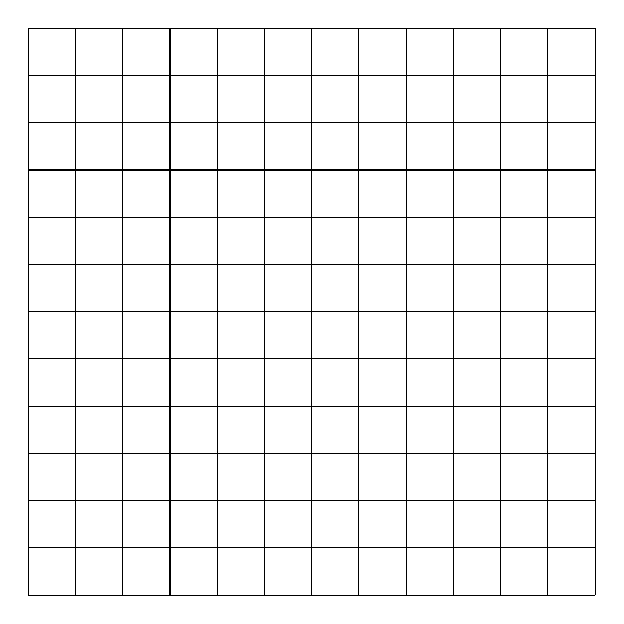
\begin{tikzpicture}%[scale=0.7]

\draw[step=0.6, black] (0,0) grid (7.2,7.2);
\node at (0.3,0.9) {\symqueen};
\node at (0.9,2.1) {\symqueen};
\node at (1.5,3.3) {\symqueen};
\node at (2.1,4.5) {\symqueen};

\node at (3.3,0.3) {\symqueen};
\node at (3.9,1.5) {\symqueen};
\node at (4.5,2.7) {\symqueen};
\node at (5.1,3.9) {\symqueen};

\node at (5.7,5.7) {\symqueen};
\node at (6.9,6.3) {\symqueen};

%\draw[thin,dashed] (0,0) -- (1,1);
%\draw[thin,dashed] (1,0) -- (1,1);
%\draw[red,thin,dashed] (2,0) -- (1,2);
%\draw[red,thin,dashed] (1,1) -- (1,2);
\end{tikzpicture} 
\caption{$10$ queens on $\mathbb{Z}_{12}^2$}
\label{case12}
\end{figure}

Finally, if $n=4$, place queens on $(0,0)$ and $(1,2)$. If $n=6$, place queens on $(0,0)$, $(1,3)$, $(2,5)$, and $(3,2)$ -- their difference values are $0,2,3,5$ and their sum values are $0,4,1,5$ in $\mathbb{Z}_6$. If $n=12$, it is easy to check visually that on Figure \ref{case12}, the set of queens is independent. \end{proof}


\end{document}
